\documentclass[letterpaper]{article}
\usepackage[T1]{fontenc}
\usepackage[utf8]{inputenc}
%\usepackage[ansinew]{inputenc}
\usepackage[spanish]{babel}
\usepackage{graphicx}
\usepackage{listings}
\title{Proyecto 2\\ Laboratorio de Microcontroladores Temporizador y GPIOs }
\author{
Marco Antonio Montero Chavarría, Carné: A94000\\
 \and
Francisco Molina, Carné: B14194\\
}

\begin{document}
\maketitle
\section{Cambios en la solución propuesta}
Se desarrolló un "semáforo inteligente" simplificado utilizando los leds, la botonera, y los temporizadores del microcontrolador STM32F4. De los cuatro leds disponibles en el microcontrolador, los leds LD3 y LD5 representarán el semáforo vehicular, mientras que los LD4 y LD6 serían el semáforo peatonal. El botón B1 (user\_button) sería el puerto con el que el usuario solicitará la activación de las luces peatonales. \\[0.5cm]

La asignación de funcionalidades de los leds es la siguiente:

\begin{itemize}
\item GPIO12 //Vehiculo Verde
\item GPIO13 //Peatonal Rojo
\item GPIO15 //Peatonal Verde
\item GPIO14 //Vehiculo Rojo
\end{itemize}

\begin{figure}[hbtp]
\centering
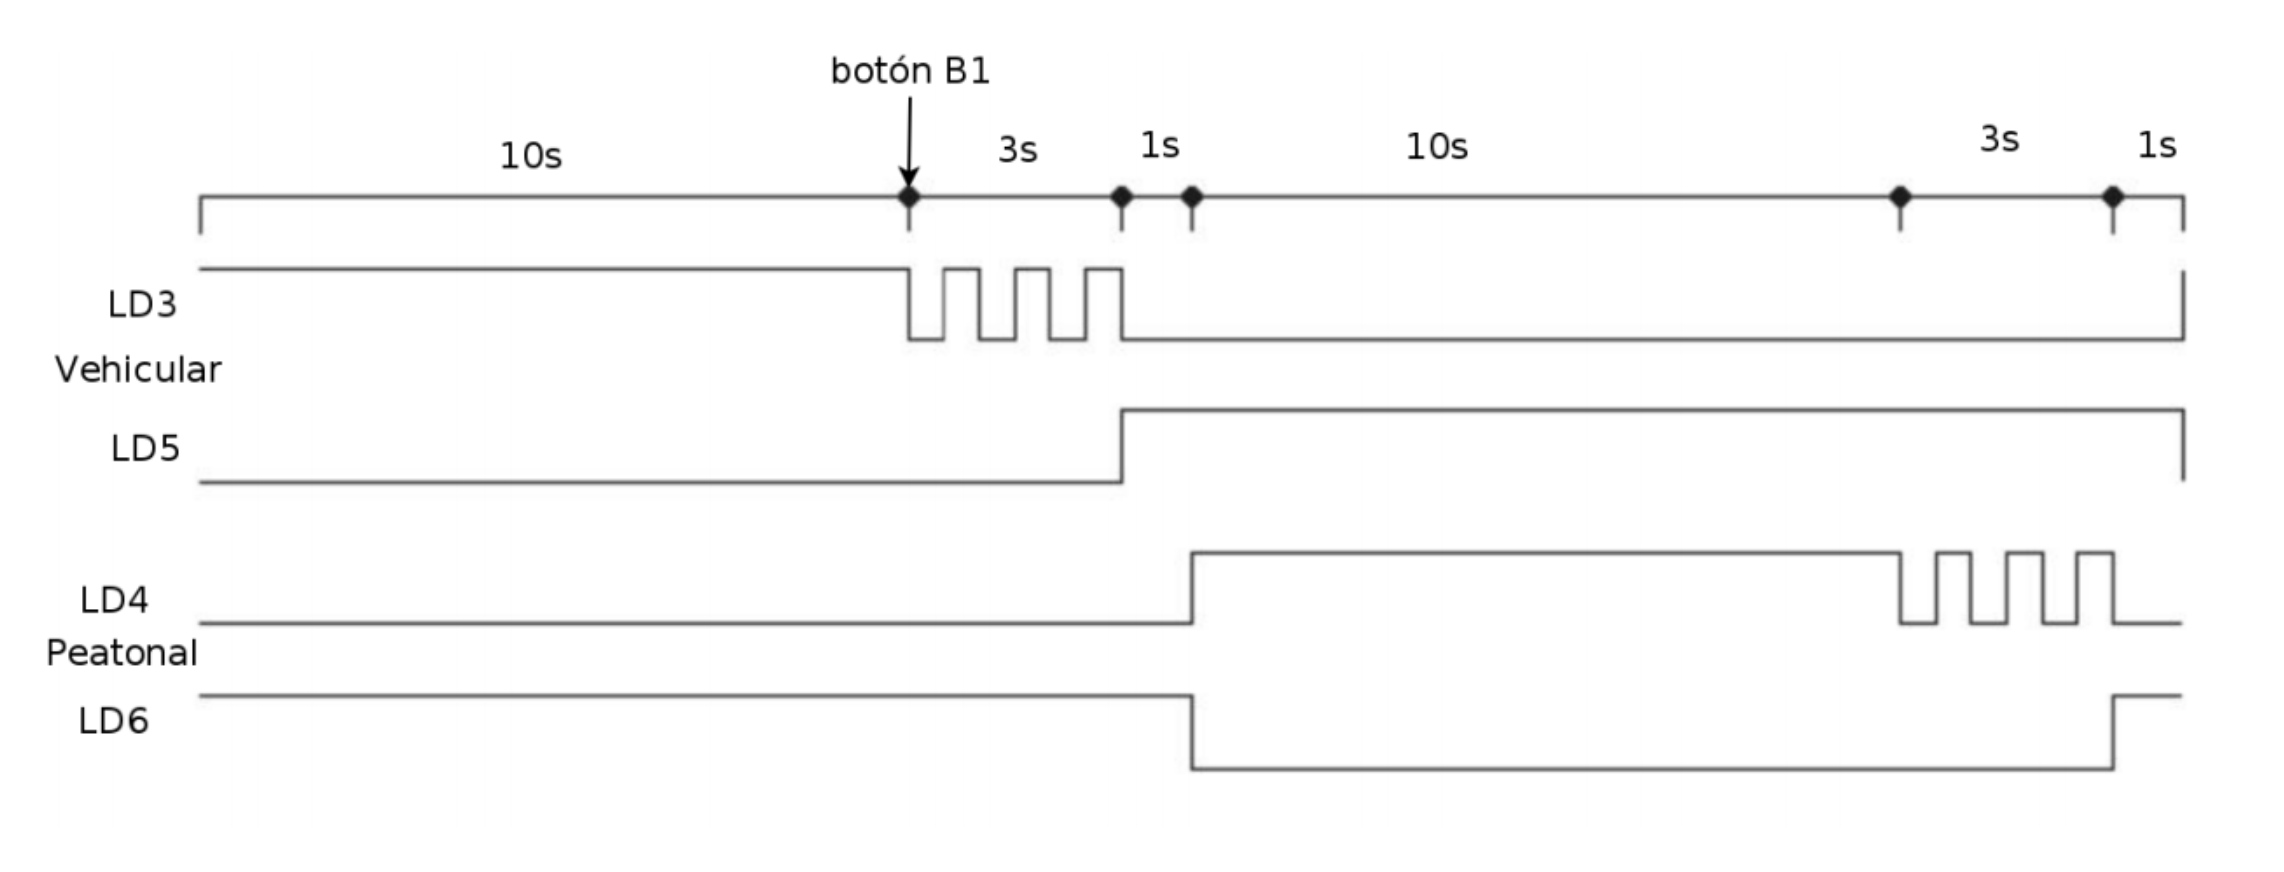
\includegraphics[width=11 cm]{tiempo1.png}
\caption{Diagrama de tiempos}
\label{semaf}
\end{figure}

Se elaboró la máquina de estados de acuerdo con el diagrama de la figura \ref{semaf}, de forma que  el botón se puede presionar inclusive antes que se acaben los 10s  del funcionamiento de LD3, pero deberá permanecer encendido hasta que terminen los 10s. Si no se presiona el botón LD3 debería permanecer encendido indefinidamente. 
La temporización de los leds se realizó utilizando el advanced timer 1 con interrupciones de tiempo habilitados, uno de los temporizadores del microcontrolador. Para esto se utilizó el archivo glove.c en la carpeta scr\_glove de opencoroco que fue modificado en el proyecto 1.\cite{coroco}  \\[0.5cm]

Como innovación se agregaron leds externos para representar adecuadamente con colores verde y rojo ambos semáforos, o agregar una luz amarilla externa con su respectivo control adicional. Se agregaron al circuito resistencias de pull-up para los leds alimentados por el mismo micro-controlador para garantizar la seguridad de la tarjeta. En el link: https://youtu.be/X7pJ6M0UVCE se puede ver el funcionamiento del semáforo en sus diferentes estados.

\section{Justificación de resultados}
Adjunto se encuentra el archivo con el código fuente de donde se toman las justificaciones. En el primer paso del video vemos como al iniciar el semáforo vehicular se encuentra en verde y el peatonal en rojo, se esperan 10 segundos antes de estripar el botón y por eso justo al estriparlo se ponen las luces en intermitente y se hace el cambio para dejar el peatonal en verde y el vehicular en rojo. Se deja un tiempo para el paso de peatones, se ponen de nuevo las luces en intermitente y se vuelve al estado inicial..\\[0.5cm]
En el segundo caso, la señal de paso del peatonal llega antes de que pasen los 10 segundos, sin embargo el semáforo al igual que en el diagrama no cambia de estado hasta que haya pasado el tiempo mínimo, con lo que se comprueba el correcto funcionamiento del mismo.\\[0.5cm]
 
\newpage

Como jutificación de ello,  los estados se definieron por medio de if's anidados, que permiten permiten incluir los retardos de tiempo necesarios entre cada una de las funciones del semáforo, como lo son el temporizador de 10 seg previo al contacto del botón para pedir paso peatonal. Este temporizador espera 10 segundos y se limpia cada vez que hay un contacto en el botón. Si el bóton llega antes de que se cumplan los 10 seg, el método funciona de tal manera que el cambio de luces se realiza hasta que se cumplan esos 10 seg mínimos.\\[0.5cm]
Además se pone una mecánica de parpadeo a los leds para indicar que van a cambiar de estado, esto se logra mediante los if's que poseen un contador interno con los métodos toggle dentro de sus llaves.\\[0.5cm]

\begin{figure}[hbtp]
\centering
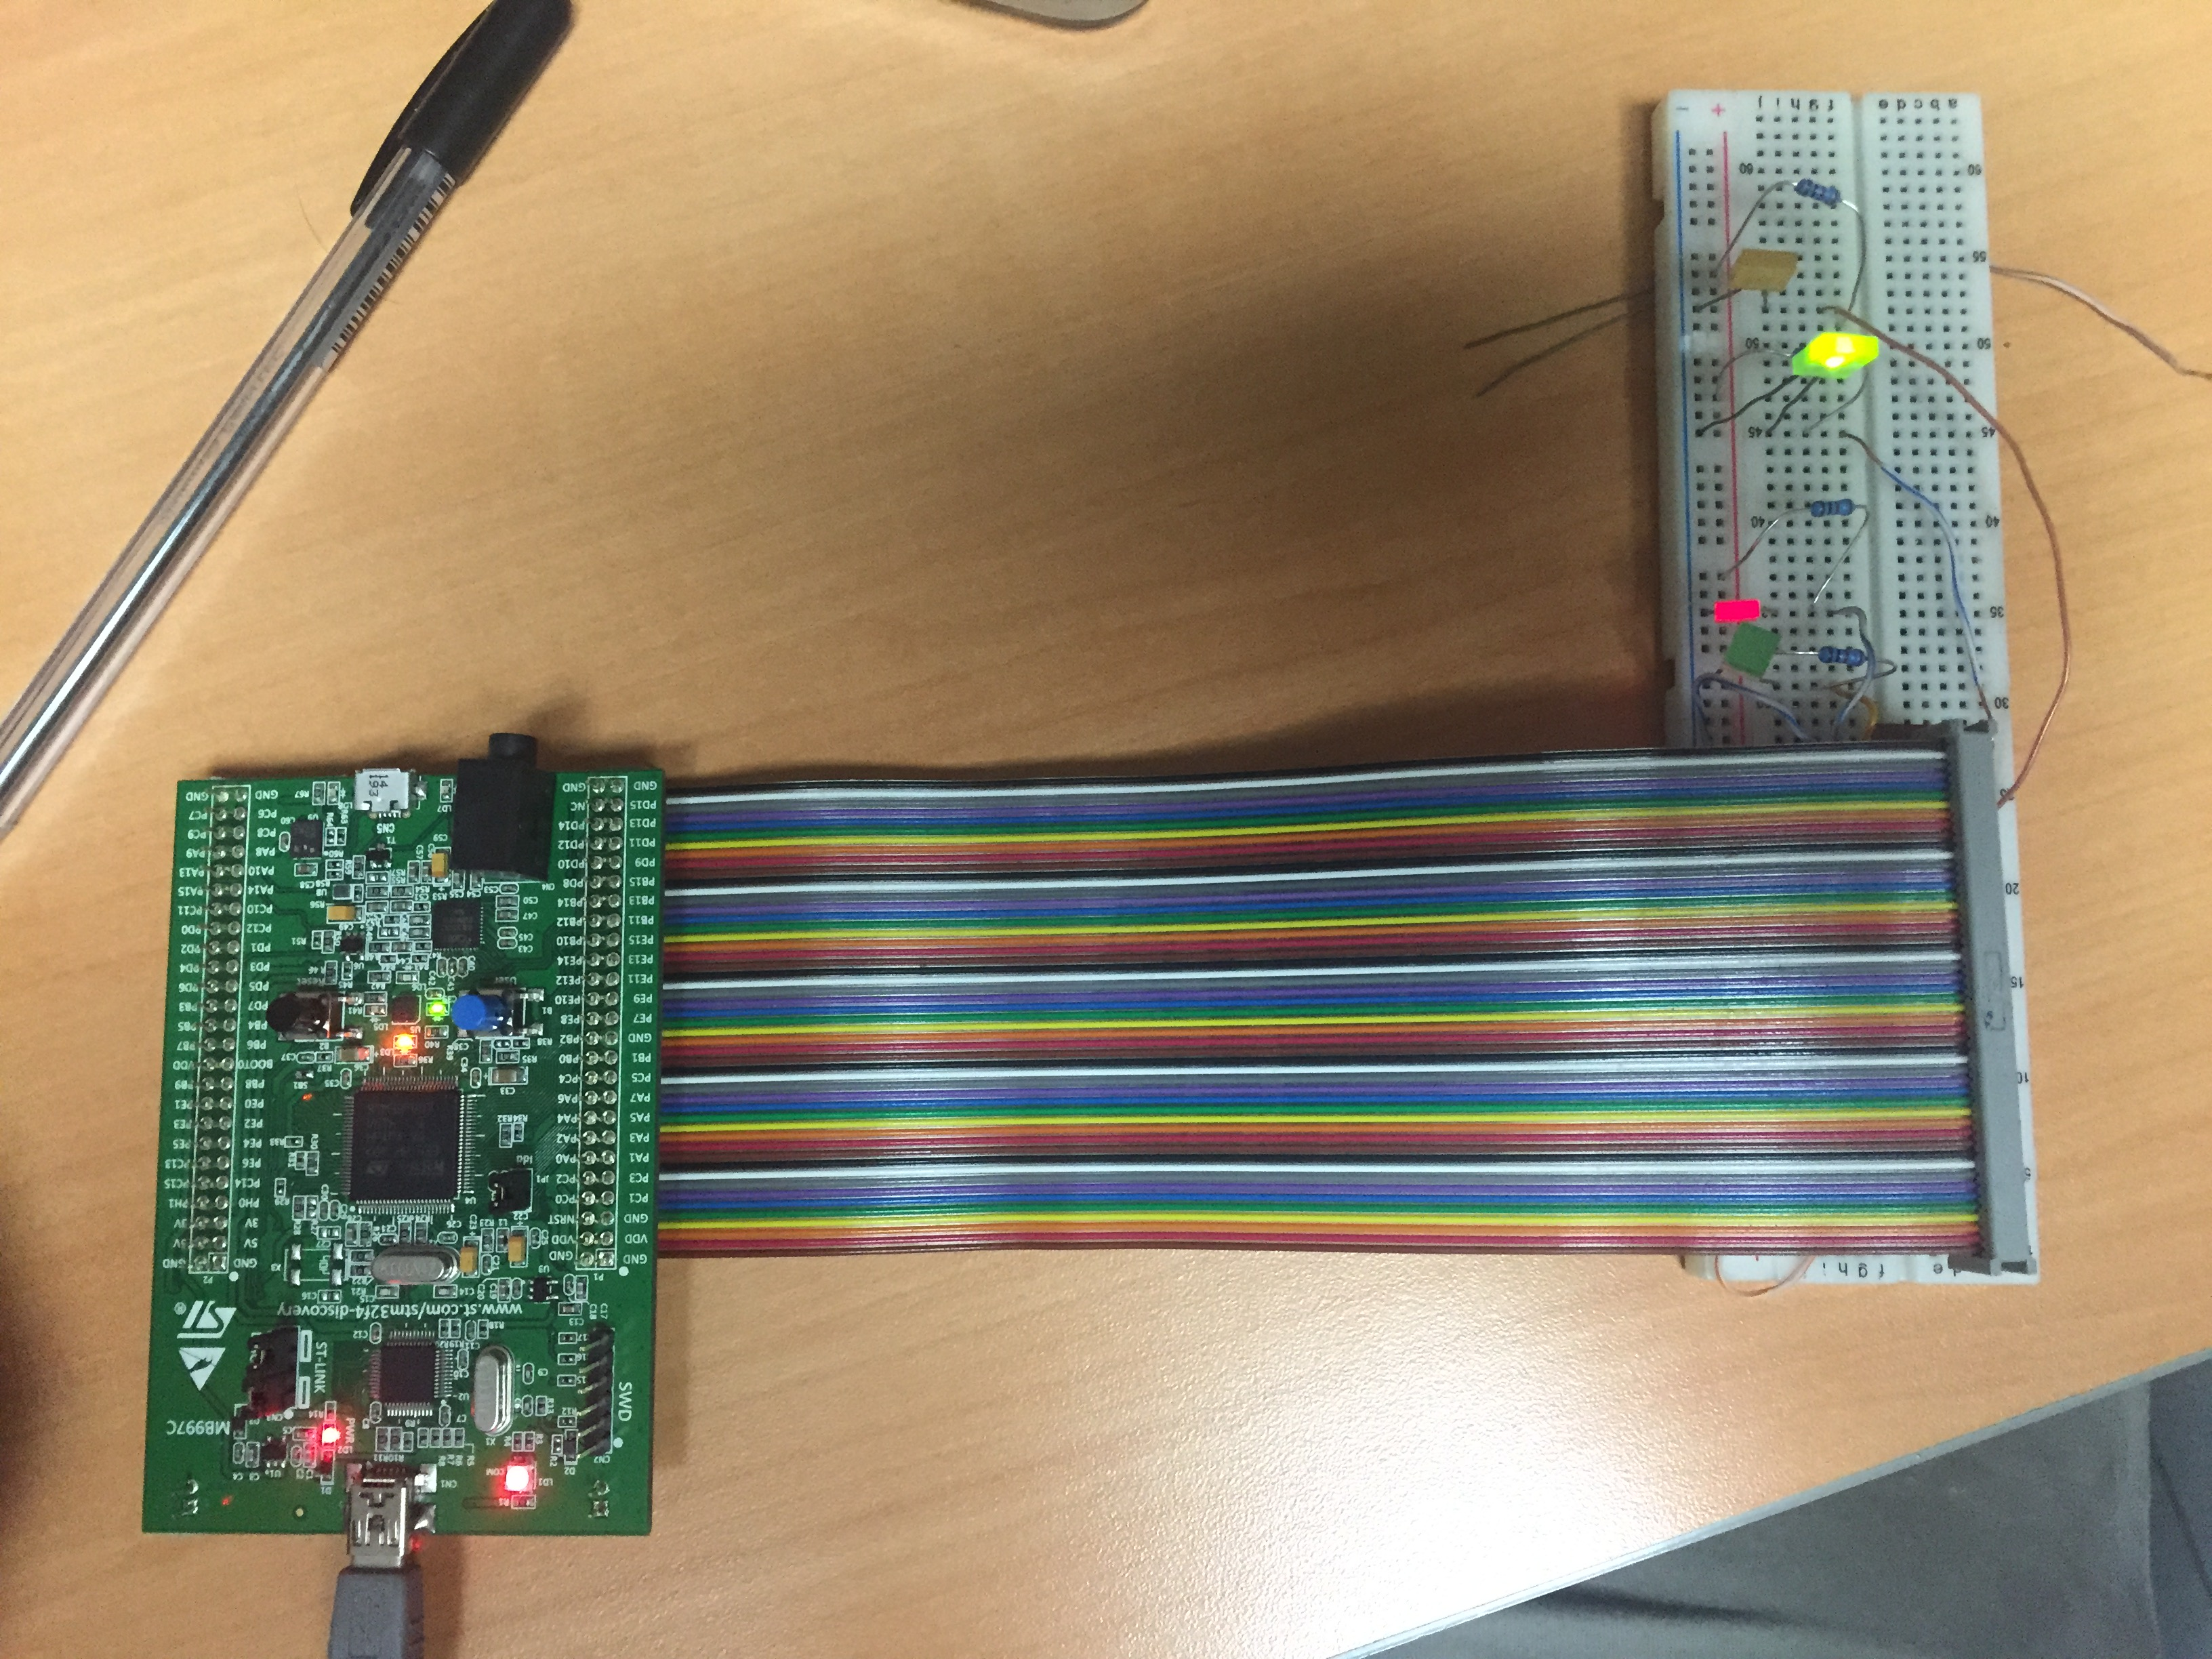
\includegraphics[width=12 cm]{fotillo.png}
\caption{Fotografía del sistema}
\label{foto}
\end{figure}

\newpage
\section{Conclusiones y recomendaciones}

El proyecto a pesar de tener sus dificultades iniciales, sirvió como introducción a la utilización del microcontrolador, así como la visualización de la forma en que se utilizan estos sistemas para diferentes tipos de proyectos. La elaboración e implementación de una máquina de estados, permitió una asimilación de materia vista en cursdos anteriores y la realización reflejó diferentes conceptos en un proyecto más palpable que la teoría. Cabe destacar que el proyecto deja una base sólida para futuros proyectos en especial el uso de temporizadores, ya que son extremadamente útiles para definir comportamientos reales con retardos. \\[0.5cm]

Como recomendaciones para futuros trabajos, se podría trabajar la complejidad aún más, quizas añadir un tercer led para el semáforo de vehículos que sea de color amarillo. Adicionalmente se puede estructurar de mejor forma el código y probar diferentes formas de lógica a la hora de realizar los condicionales. 



\bibliographystyle{alpha} 
\bibliography{refs}



\end{document}
